\section{Dataset Description}

\subsection{Overview}

We use the \textbf{Corona NLP} dataset \cite{datatattle2020coronanlp}, originally published on Kaggle by Datatattle and made available under the MIT licence. The dataset consists of tweets collected from Twitter during the early months of the COVID-19 pandemic (March--April 2020) and annotated with one of five sentiment labels.

The dataset is supplied in two pre-defined splits:
\begin{itemize}
    \item \textbf{Training set:} 41,157 samples (\path{Corona_NLP_train.csv})
    \item \textbf{Test set:} 3,798 samples (\path{Corona_NLP_test.csv})
\end{itemize}

Each record contains the following columns: \texttt{UserName}, \texttt{ScreenName}, \texttt{Location}, \texttt{TweetAt}, \texttt{OriginalTweet}, and \texttt{Sentiment}. Only \texttt{OriginalTweet} (the input) and \texttt{Sentiment} (the label) are used during training and evaluation.

\subsection{Label Distribution}

The five sentiment classes and their distributions in the official training split are reported in Table~\ref{tab:class_distribution}.

\begin{table}[H]
    \centering
    \caption{Class distribution in the Corona NLP training split (41,157 samples).}
    \label{tab:class_distribution}
    \begin{tabularx}{\textwidth}{l r r}
        \toprule
        \textbf{Sentiment Class} & \textbf{Count} & \textbf{Percentage (\%)} \\
        \midrule
        Extremely Negative & 5,481  & 13.32 \\
        Negative           & 8,500  & 20.65 \\
        Neutral            & 7,713  & 18.74 \\
        Positive           & 11,422 & 27.75 \\
        Extremely Positive & 8,041  & 19.54 \\
        \midrule
        \textbf{Total}     & \textbf{41,157} & \textbf{100.00} \\
        \bottomrule
    \end{tabularx}
\end{table}

The dataset is \textbf{moderately imbalanced}: the \textit{Positive} class is the most frequent (27.75\%) while \textit{Extremely Negative} is the least frequent (13.32\%), giving a max-to-min ratio of approximately 2.1:1. While not severe, this imbalance motivates the use of \textbf{macro-averaged F1} as the primary evaluation metric, which treats all classes equally regardless of support.

\begin{figure}[H]
    \centering
    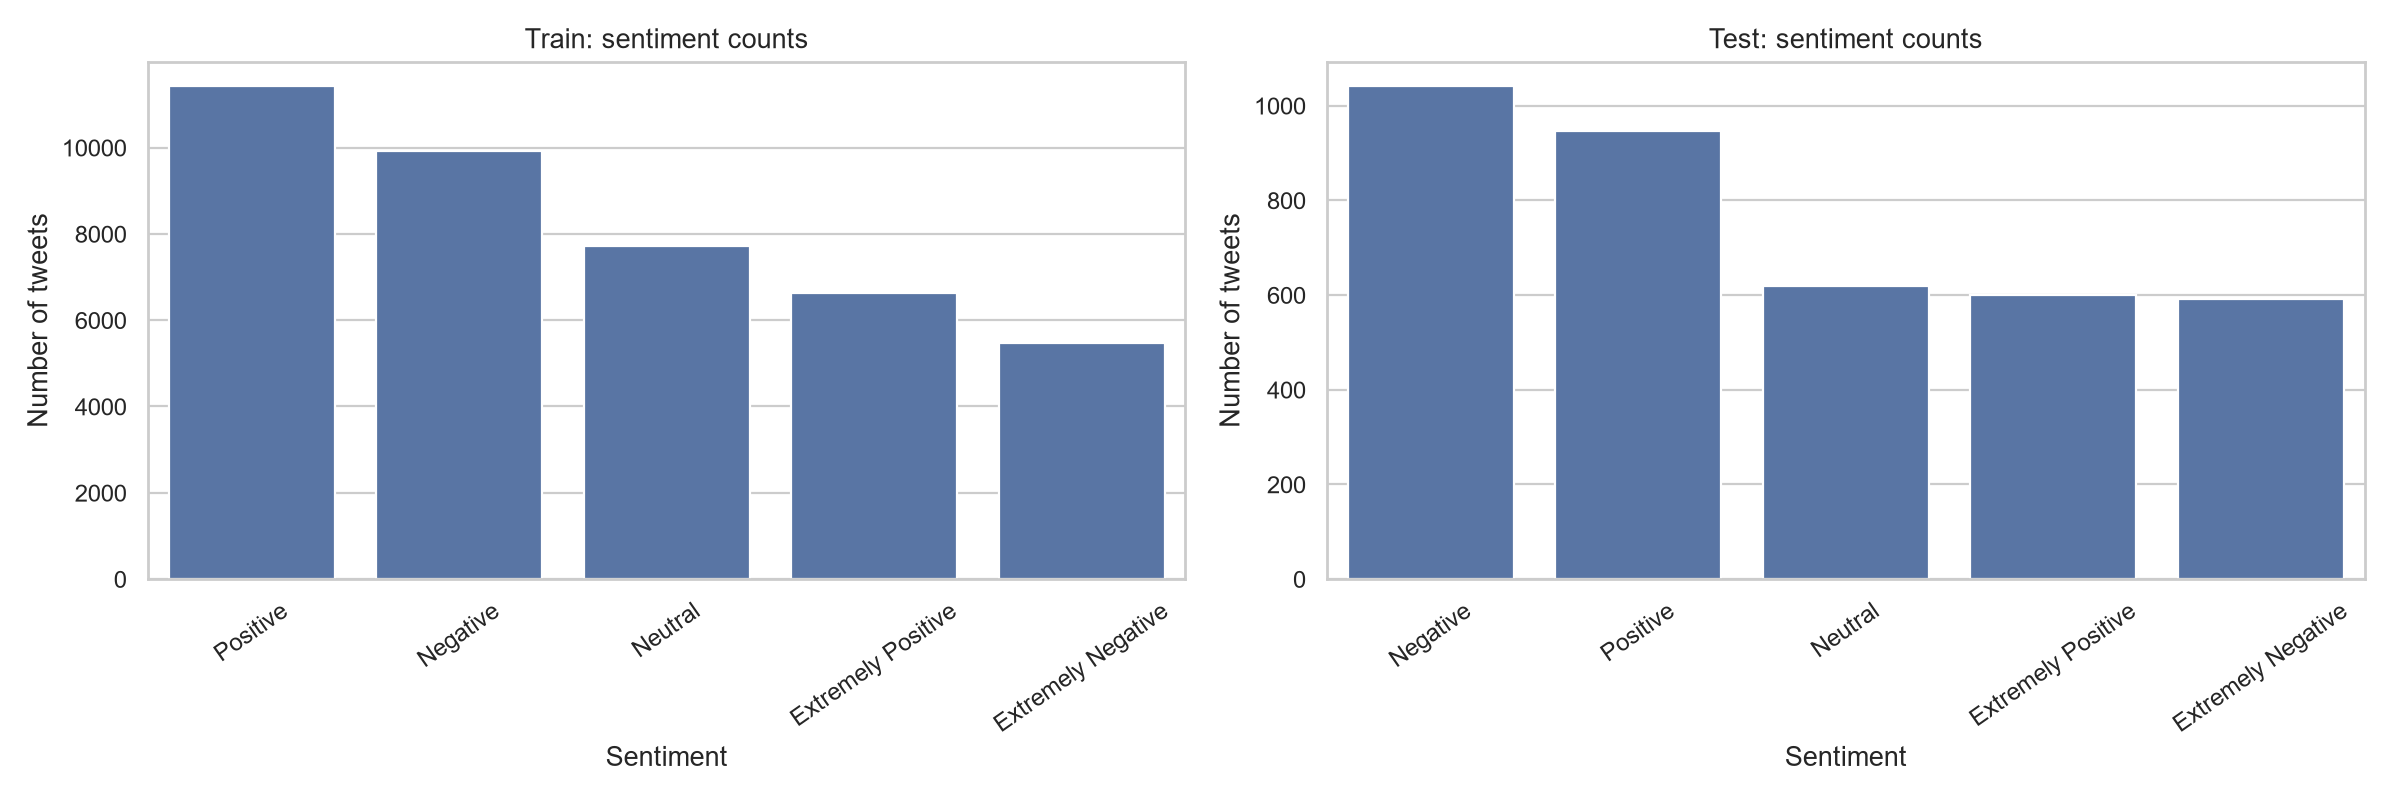
\includegraphics[width=0.70\textwidth]{../../Assignment2/corona_eda/class_distribution.png}
    \caption{Bar chart of class distribution in the Corona NLP training split.}
    \label{fig:class_distribution}
\end{figure}

\subsection{Sample Tweets}

Figure~\ref{fig:random_examples} shows a selection of randomly sampled tweets from the training set, illustrating the diversity of language style, topic coverage, and sentiment expression. Tweets frequently contain informal constructs such as hashtags (\texttt{\#coronavirus}), user mentions (\texttt{@realDonaldTrump}), URLs, and emoji, all of which challenge standard NLP pipelines.

\begin{figure}[H]
    \centering
    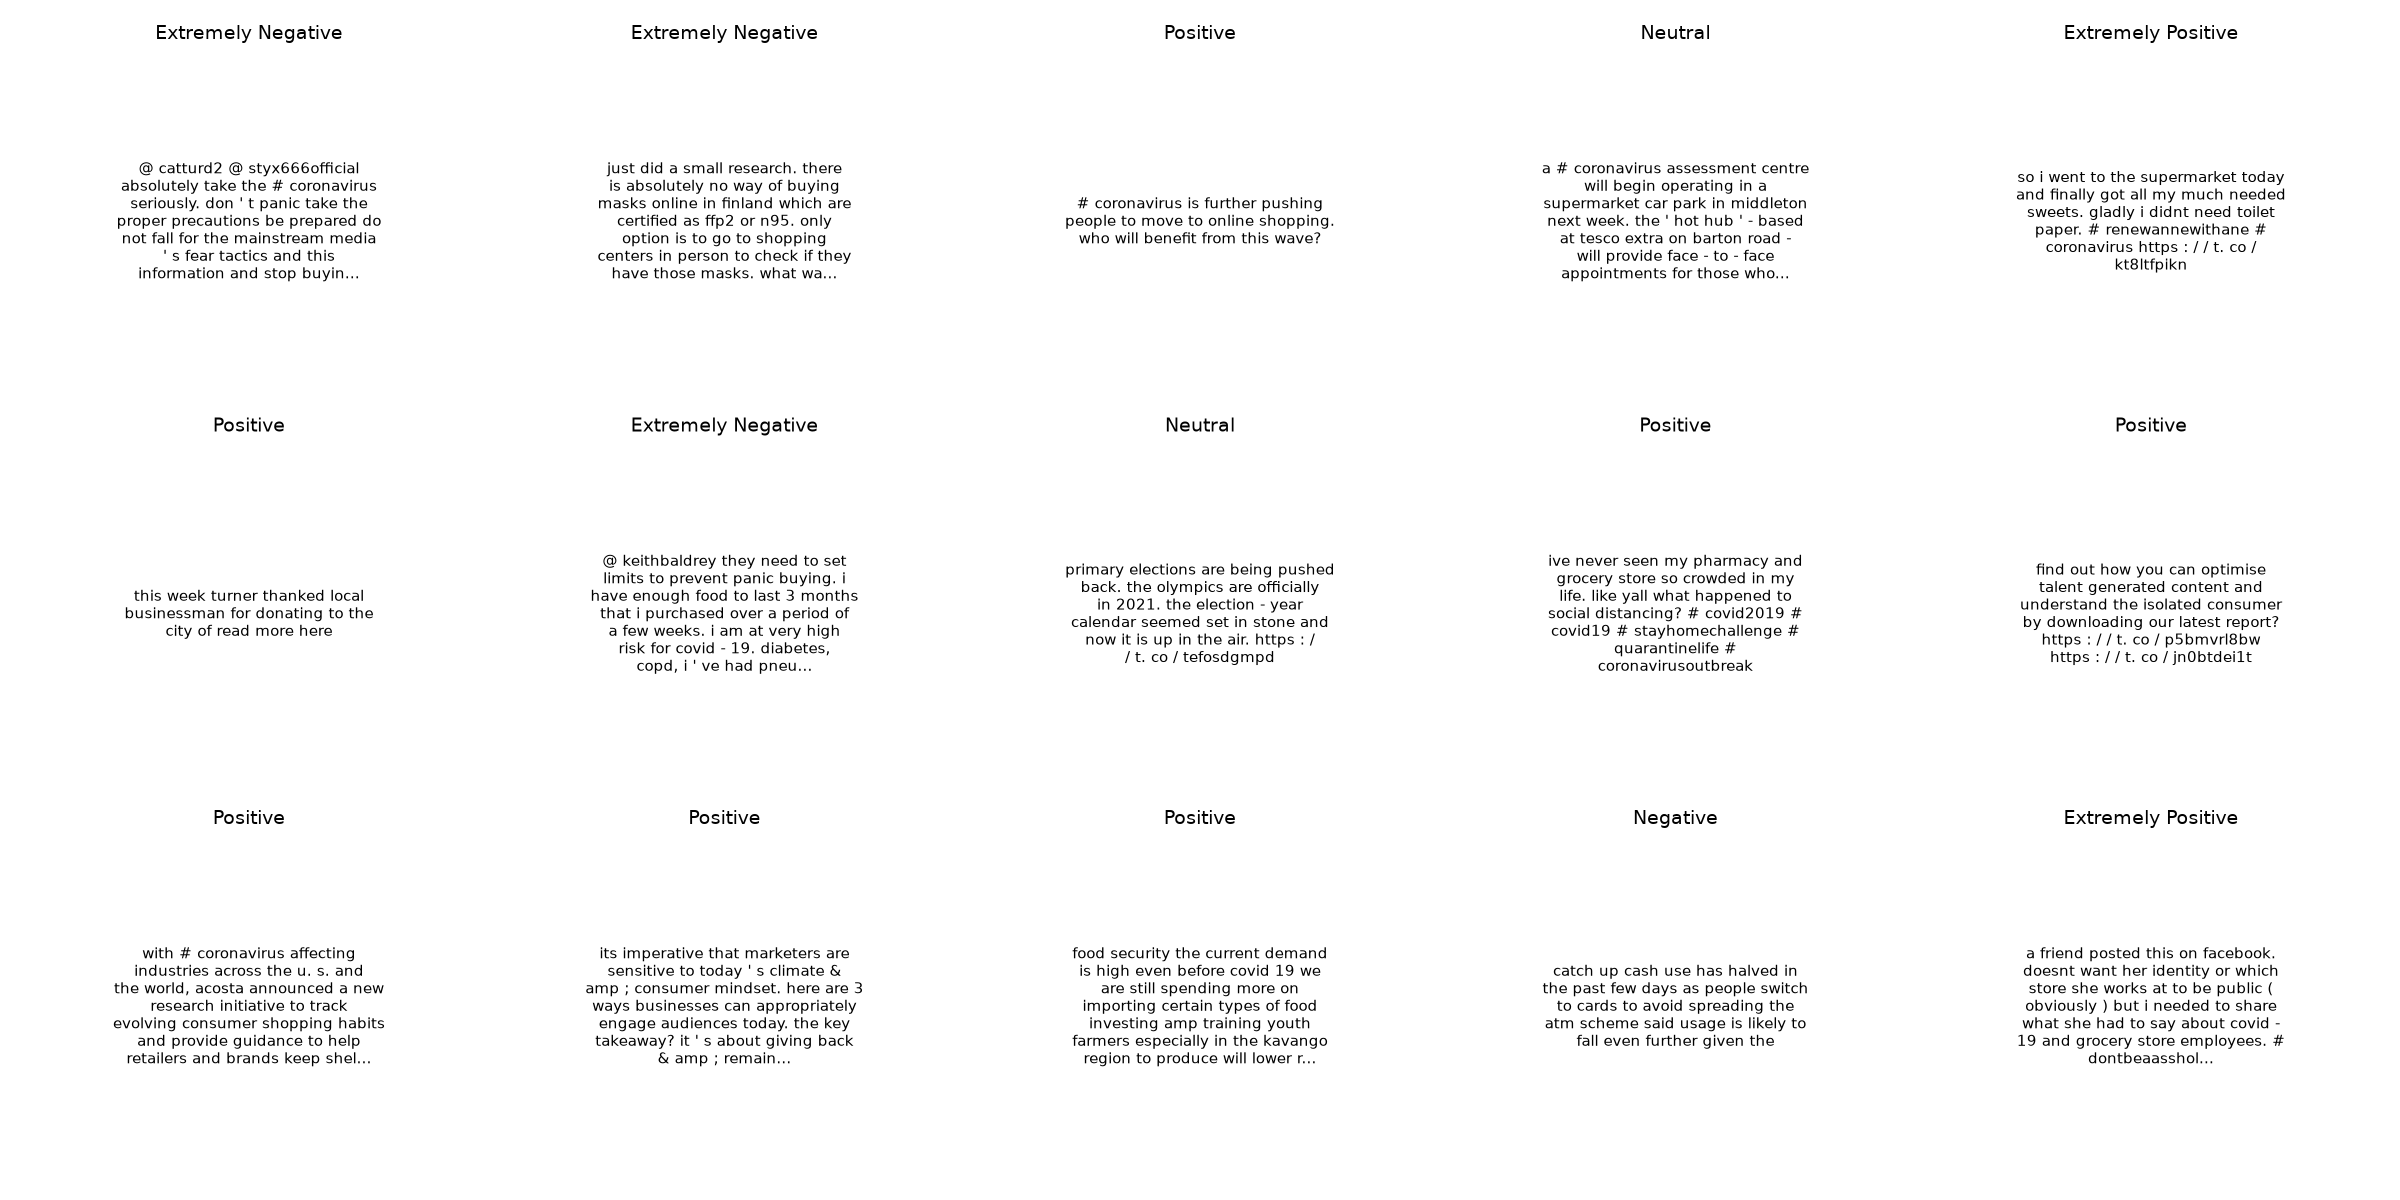
\includegraphics[width=\textwidth]{../../Assignment2/outputs/eda/random_examples.png}
    \caption{Randomly sampled tweets from the training set, grouped by sentiment class.}
    \label{fig:random_examples}
\end{figure}

\subsection{Data Quality Notes}

A deduplication scan of the training set revealed 15 exact duplicate rows (same tweet text appearing more than once). Additionally, 1 tweet appears in both the training and the official test file, representing a cross-split overlap of 0.026\% of the test set. These issues are minor and no rows were removed; they are reported for completeness and reproducibility.
